\documentclass{standalone}
\usepackage[all]{xy}
\usepackage{bm}
\usepackage{tikz}

\usetikzlibrary{shapes.arrows, shapes.geometric}
\tikzstyle{line} = [thick,->]
\tikzstyle{arrow} = [
	thick,
	->,
	>=stealth,
	black,
]
\tikzstyle{agente} = [
	rectangle, 
	minimum width=1cm, 
	minimum height=1cm,
	text centered,
	draw=black, 
	fill=green!30
]
\tikzstyle{modelo} = [
	rectangle, 
	rounded corners,
	minimum width=1cm, 
	minimum height=1cm,
	text centered,
	draw=black, 
	fill=red!30
]
\tikzstyle{memoria} = [
	rectangle, 
	rounded corners,
	minimum width=1cm, 
	minimum height=1cm,
	text centered,
	draw=black, 
	fill=gray!30
]
\tikzstyle{entorno} = [
	rectangle, 
	minimum width=1cm, 
	minimum height=1cm,
	text centered, 
	draw=black, 
	fill=blue!15
]


\begin{document}

\begin{tikzpicture}
\node(A) at (0,4) {\txt{History\\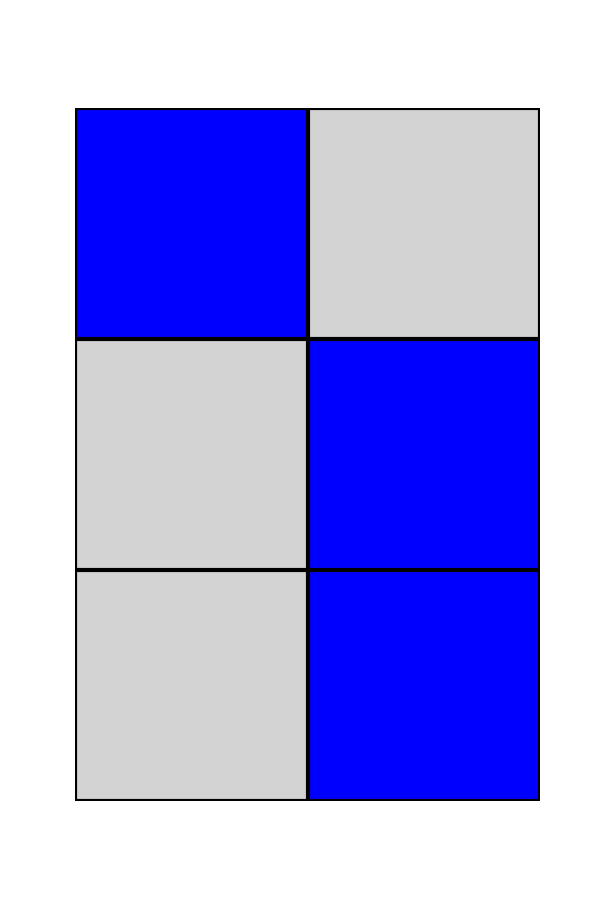
\includegraphics[width=2cm]{history_1.png}\\len=2}};
\node(B) at (-4,0) {\txt{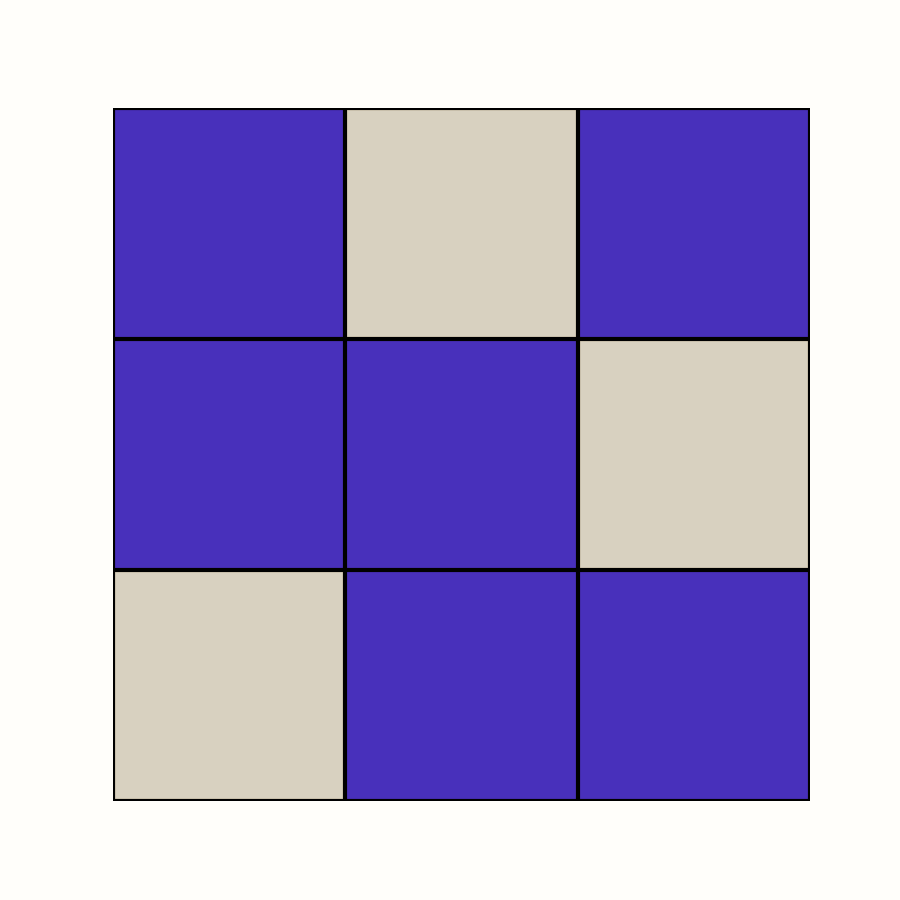
\includegraphics[width=3cm]{FRA_region_1.png}\\Focal Schemata}};
\node(C1) at (-4.5, 1.65) {};

\node(M) at (-3, 4.75) {player 1};
\node(Mh1) at (-1, 4.75) {};
\draw [->] (M) -- (Mh1);

\draw [black!83, thick, dashed] (-5.2, 1.4) rectangle (-3.5,-1);
\draw[arrow, black!83, line width=1.5pt] (A) edge [out=180, in=90, anchor=south east] node {Jacc.Sim.$=0.83$} (C1);

\node(D1) at (-3.2, 1) {};
\node(D2) at (-0.6, -2.5) {\{don't go=0.17, go=0.83\}};
\draw[black, line width=1.5pt, ->] (D1) edge [out=0, in=90] (D2);

\node(S) at (3.5, -3.5) {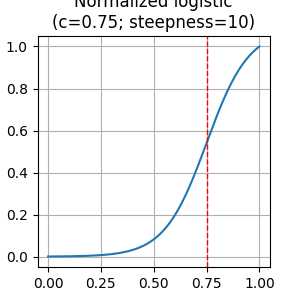
\includegraphics[width=3cm]{logistic.png}};

\node(BD2) at (5, 0) {\{don't go=0, go=1\}};
\draw[black, line width=1.5pt, ->] (D2) edge [out=30, in=270] (BD2);

\node(1) at (-1.5, 5.5) {\textbf{I}};
\node(2) at (-4.5, 4.2) {\textbf{II}};
\node(3) at (-0.5, 0) {\textbf{III}};
\node(4) at (5.5, -3.5) {\textbf{IV}};


\end{tikzpicture}

\end{document}